\documentclass[]{article}
\usepackage{lmodern}
\usepackage{amssymb,amsmath}
\usepackage{ifxetex,ifluatex}
\usepackage{fixltx2e} % provides \textsubscript
\ifnum 0\ifxetex 1\fi\ifluatex 1\fi=0 % if pdftex
  \usepackage[T1]{fontenc}
  \usepackage[utf8]{inputenc}
\else % if luatex or xelatex
  \ifxetex
    \usepackage{mathspec}
  \else
    \usepackage{fontspec}
  \fi
  \defaultfontfeatures{Ligatures=TeX,Scale=MatchLowercase}
\fi
% use upquote if available, for straight quotes in verbatim environments
\IfFileExists{upquote.sty}{\usepackage{upquote}}{}
% use microtype if available
\IfFileExists{microtype.sty}{%
\usepackage{microtype}
\UseMicrotypeSet[protrusion]{basicmath} % disable protrusion for tt fonts
}{}
\usepackage[margin=1in]{geometry}
\usepackage{hyperref}
\hypersetup{unicode=true,
            pdftitle={Scoring Evaluations},
            pdfauthor={Dave Bridges},
            pdfborder={0 0 0},
            breaklinks=true}
\urlstyle{same}  % don't use monospace font for urls
\usepackage{color}
\usepackage{fancyvrb}
\newcommand{\VerbBar}{|}
\newcommand{\VERB}{\Verb[commandchars=\\\{\}]}
\DefineVerbatimEnvironment{Highlighting}{Verbatim}{commandchars=\\\{\}}
% Add ',fontsize=\small' for more characters per line
\usepackage{framed}
\definecolor{shadecolor}{RGB}{248,248,248}
\newenvironment{Shaded}{\begin{snugshade}}{\end{snugshade}}
\newcommand{\KeywordTok}[1]{\textcolor[rgb]{0.13,0.29,0.53}{\textbf{#1}}}
\newcommand{\DataTypeTok}[1]{\textcolor[rgb]{0.13,0.29,0.53}{#1}}
\newcommand{\DecValTok}[1]{\textcolor[rgb]{0.00,0.00,0.81}{#1}}
\newcommand{\BaseNTok}[1]{\textcolor[rgb]{0.00,0.00,0.81}{#1}}
\newcommand{\FloatTok}[1]{\textcolor[rgb]{0.00,0.00,0.81}{#1}}
\newcommand{\ConstantTok}[1]{\textcolor[rgb]{0.00,0.00,0.00}{#1}}
\newcommand{\CharTok}[1]{\textcolor[rgb]{0.31,0.60,0.02}{#1}}
\newcommand{\SpecialCharTok}[1]{\textcolor[rgb]{0.00,0.00,0.00}{#1}}
\newcommand{\StringTok}[1]{\textcolor[rgb]{0.31,0.60,0.02}{#1}}
\newcommand{\VerbatimStringTok}[1]{\textcolor[rgb]{0.31,0.60,0.02}{#1}}
\newcommand{\SpecialStringTok}[1]{\textcolor[rgb]{0.31,0.60,0.02}{#1}}
\newcommand{\ImportTok}[1]{#1}
\newcommand{\CommentTok}[1]{\textcolor[rgb]{0.56,0.35,0.01}{\textit{#1}}}
\newcommand{\DocumentationTok}[1]{\textcolor[rgb]{0.56,0.35,0.01}{\textbf{\textit{#1}}}}
\newcommand{\AnnotationTok}[1]{\textcolor[rgb]{0.56,0.35,0.01}{\textbf{\textit{#1}}}}
\newcommand{\CommentVarTok}[1]{\textcolor[rgb]{0.56,0.35,0.01}{\textbf{\textit{#1}}}}
\newcommand{\OtherTok}[1]{\textcolor[rgb]{0.56,0.35,0.01}{#1}}
\newcommand{\FunctionTok}[1]{\textcolor[rgb]{0.00,0.00,0.00}{#1}}
\newcommand{\VariableTok}[1]{\textcolor[rgb]{0.00,0.00,0.00}{#1}}
\newcommand{\ControlFlowTok}[1]{\textcolor[rgb]{0.13,0.29,0.53}{\textbf{#1}}}
\newcommand{\OperatorTok}[1]{\textcolor[rgb]{0.81,0.36,0.00}{\textbf{#1}}}
\newcommand{\BuiltInTok}[1]{#1}
\newcommand{\ExtensionTok}[1]{#1}
\newcommand{\PreprocessorTok}[1]{\textcolor[rgb]{0.56,0.35,0.01}{\textit{#1}}}
\newcommand{\AttributeTok}[1]{\textcolor[rgb]{0.77,0.63,0.00}{#1}}
\newcommand{\RegionMarkerTok}[1]{#1}
\newcommand{\InformationTok}[1]{\textcolor[rgb]{0.56,0.35,0.01}{\textbf{\textit{#1}}}}
\newcommand{\WarningTok}[1]{\textcolor[rgb]{0.56,0.35,0.01}{\textbf{\textit{#1}}}}
\newcommand{\AlertTok}[1]{\textcolor[rgb]{0.94,0.16,0.16}{#1}}
\newcommand{\ErrorTok}[1]{\textcolor[rgb]{0.64,0.00,0.00}{\textbf{#1}}}
\newcommand{\NormalTok}[1]{#1}
\usepackage{longtable,booktabs}
\usepackage{graphicx,grffile}
\makeatletter
\def\maxwidth{\ifdim\Gin@nat@width>\linewidth\linewidth\else\Gin@nat@width\fi}
\def\maxheight{\ifdim\Gin@nat@height>\textheight\textheight\else\Gin@nat@height\fi}
\makeatother
% Scale images if necessary, so that they will not overflow the page
% margins by default, and it is still possible to overwrite the defaults
% using explicit options in \includegraphics[width, height, ...]{}
\setkeys{Gin}{width=\maxwidth,height=\maxheight,keepaspectratio}
\IfFileExists{parskip.sty}{%
\usepackage{parskip}
}{% else
\setlength{\parindent}{0pt}
\setlength{\parskip}{6pt plus 2pt minus 1pt}
}
\setlength{\emergencystretch}{3em}  % prevent overfull lines
\providecommand{\tightlist}{%
  \setlength{\itemsep}{0pt}\setlength{\parskip}{0pt}}
\setcounter{secnumdepth}{0}
% Redefines (sub)paragraphs to behave more like sections
\ifx\paragraph\undefined\else
\let\oldparagraph\paragraph
\renewcommand{\paragraph}[1]{\oldparagraph{#1}\mbox{}}
\fi
\ifx\subparagraph\undefined\else
\let\oldsubparagraph\subparagraph
\renewcommand{\subparagraph}[1]{\oldsubparagraph{#1}\mbox{}}
\fi

%%% Use protect on footnotes to avoid problems with footnotes in titles
\let\rmarkdownfootnote\footnote%
\def\footnote{\protect\rmarkdownfootnote}

%%% Change title format to be more compact
\usepackage{titling}

% Create subtitle command for use in maketitle
\newcommand{\subtitle}[1]{
  \posttitle{
    \begin{center}\large#1\end{center}
    }
}

\setlength{\droptitle}{-2em}
  \title{Scoring Evaluations}
  \pretitle{\vspace{\droptitle}\centering\huge}
  \posttitle{\par}
  \author{Dave Bridges}
  \preauthor{\centering\large\emph}
  \postauthor{\par}
  \predate{\centering\large\emph}
  \postdate{\par}
  \date{1/31/2018}


\begin{document}
\maketitle

{
\setcounter{tocdepth}{2}
\tableofcontents
}
\subsection{Data Import}\label{data-import}

Exported \textbf{Assignment Type Summaries} from GradeCraft and
imported.

\begin{Shaded}
\begin{Highlighting}[]
\KeywordTok{library}\NormalTok{(readr)}
\KeywordTok{library}\NormalTok{(dplyr)}
\KeywordTok{library}\NormalTok{(tidyr)}
\NormalTok{datafile <-}\StringTok{ 'Principles of Nutritional Sciences Assignment Type Summary - 2018-02-01.csv'}

\KeywordTok{library}\NormalTok{(readr)}
\NormalTok{dataset <-}\StringTok{ }\KeywordTok{read_csv}\NormalTok{(datafile)}

\NormalTok{dropped.students <-}\StringTok{ }\KeywordTok{c}\NormalTok{(}\StringTok{'dave.bridges'}\NormalTok{,}\StringTok{'ajian'}\NormalTok{,}\StringTok{'zhongyli'}\NormalTok{)}

\NormalTok{assessment.dataset <-}
\StringTok{  }\NormalTok{dataset }\OperatorTok
\StringTok{  }\KeywordTok{select}\NormalTok{(}\OperatorTok{-}\StringTok{`}\DataTypeTok{First Name}\StringTok{`}\NormalTok{, }\OperatorTok{-}\StringTok{`}\DataTypeTok{Last Name}\StringTok{`}\NormalTok{, }\OperatorTok{-}\NormalTok{Email, }\OperatorTok{-}\NormalTok{Team) }\OperatorTok
\StringTok{  }\KeywordTok{gather}\NormalTok{(Assignment, Points, }\OperatorTok{-}\NormalTok{Username) }\OperatorTok\StringTok{ }
\StringTok{  }\KeywordTok{filter}\NormalTok{(}\OperatorTok{!}\NormalTok{(Username }\OperatorTok\StringTok{ }\NormalTok{dropped.students)) }\OperatorTok
\StringTok{  }\KeywordTok{arrange}\NormalTok{(Points)}

\NormalTok{summary.dataset <-}
\StringTok{  }\NormalTok{assessment.dataset }\OperatorTok
\StringTok{  }\KeywordTok{group_by}\NormalTok{(Username) }\OperatorTok
\StringTok{  }\KeywordTok{summarize}\NormalTok{(}\DataTypeTok{Total =} \KeywordTok{sum}\NormalTok{(Points)) }\OperatorTok
\StringTok{  }\KeywordTok{arrange}\NormalTok{(}\OperatorTok{-}\NormalTok{Total)}
\end{Highlighting}
\end{Shaded}

This script imports the data from \textbf{Principles of Nutritional
Sciences Assignment Type Summary - 2018-02-01.csv}. This script is
located at
/Users/davebrid/Documents/GitHub/TeachingLectures/Michigan/NUTR630/Evaluation/GradeCraft
Summary/GradeCraft Metrics and was most recently run on Tue Feb 27
10:27:22 2018

\begin{Shaded}
\begin{Highlighting}[]
\KeywordTok{library}\NormalTok{(ggplot2)}

\NormalTok{p <-}\StringTok{ }\KeywordTok{ggplot}\NormalTok{(}\DataTypeTok{data=}\NormalTok{summary.dataset, }\KeywordTok{aes}\NormalTok{(}\DataTypeTok{x=}\NormalTok{Total)) }
\NormalTok{p }\OperatorTok{+}\StringTok{ }\KeywordTok{geom_histogram}\NormalTok{(}\DataTypeTok{binwidth=}\DecValTok{50}\NormalTok{) }\OperatorTok{+}
\StringTok{  }\KeywordTok{labs}\NormalTok{(}\DataTypeTok{x=}\StringTok{"Final Points"}\NormalTok{,}\DataTypeTok{y=}\StringTok{"Number of Students"}\NormalTok{, }\DataTypeTok{title=}\StringTok{"Distribution of Final Points"}\NormalTok{) }\OperatorTok{+}
\StringTok{  }\KeywordTok{geom_vline}\NormalTok{(}\KeywordTok{aes}\NormalTok{(}\DataTypeTok{xintercept=}\DecValTok{1000}\NormalTok{), }\DataTypeTok{color=}\StringTok{"red"}\NormalTok{, }\DataTypeTok{linetype=}\StringTok{"dashed"}\NormalTok{, }\DataTypeTok{size=}\DecValTok{1}\NormalTok{) }\OperatorTok{+}
\StringTok{  }\KeywordTok{geom_vline}\NormalTok{(}\KeywordTok{aes}\NormalTok{(}\DataTypeTok{xintercept=}\DecValTok{950}\NormalTok{), }\DataTypeTok{color=}\StringTok{"red"}\NormalTok{, }\DataTypeTok{linetype=}\StringTok{"dashed"}\NormalTok{, }\DataTypeTok{size=}\FloatTok{0.5}\NormalTok{) }\OperatorTok{+}
\StringTok{  }\KeywordTok{geom_vline}\NormalTok{(}\KeywordTok{aes}\NormalTok{(}\DataTypeTok{xintercept=}\DecValTok{900}\NormalTok{), }\DataTypeTok{color=}\StringTok{"red"}\NormalTok{, }\DataTypeTok{linetype=}\StringTok{"dashed"}\NormalTok{, }\DataTypeTok{size=}\FloatTok{0.5}\NormalTok{) }\OperatorTok{+}
\StringTok{  }\KeywordTok{geom_vline}\NormalTok{(}\KeywordTok{aes}\NormalTok{(}\DataTypeTok{xintercept=}\DecValTok{850}\NormalTok{), }\DataTypeTok{color=}\StringTok{"red"}\NormalTok{, }\DataTypeTok{linetype=}\StringTok{"dashed"}\NormalTok{, }\DataTypeTok{size=}\FloatTok{0.5}\NormalTok{) }\OperatorTok{+}
\StringTok{  }\KeywordTok{geom_vline}\NormalTok{(}\KeywordTok{aes}\NormalTok{(}\DataTypeTok{xintercept=}\DecValTok{800}\NormalTok{), }\DataTypeTok{color=}\StringTok{"red"}\NormalTok{, }\DataTypeTok{linetype=}\StringTok{"dashed"}\NormalTok{, }\DataTypeTok{size=}\FloatTok{0.5}\NormalTok{) }\OperatorTok{+}
\StringTok{  }\KeywordTok{geom_vline}\NormalTok{(}\KeywordTok{aes}\NormalTok{(}\DataTypeTok{xintercept=}\DecValTok{750}\NormalTok{), }\DataTypeTok{color=}\StringTok{"red"}\NormalTok{, }\DataTypeTok{linetype=}\StringTok{"dashed"}\NormalTok{, }\DataTypeTok{size=}\FloatTok{0.5}\NormalTok{) }\OperatorTok{+}
\StringTok{  }\KeywordTok{geom_vline}\NormalTok{(}\KeywordTok{aes}\NormalTok{(}\DataTypeTok{xintercept=}\DecValTok{700}\NormalTok{), }\DataTypeTok{color=}\StringTok{"red"}\NormalTok{, }\DataTypeTok{linetype=}\StringTok{"dashed"}\NormalTok{, }\DataTypeTok{size=}\FloatTok{0.5}\NormalTok{) }
\end{Highlighting}
\end{Shaded}

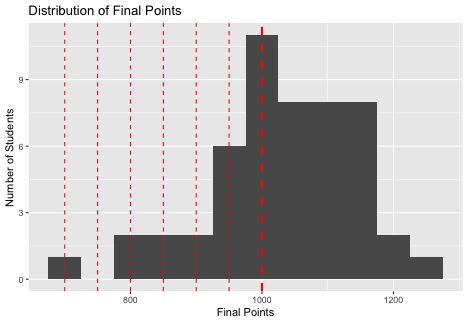
\includegraphics{figures/points-distribution-1.png}

There were 31 students who earned an A. Among those who earned an A,
their average points were 1096.419. This means that the A students
averaged \textbf{96.419} points too many than they needed. This is
relative to the overall mean of 1028.255

\subsection{Assessment Choices}\label{assessment-choices}

\subsubsection{Aggregated}\label{aggregated}

\begin{Shaded}
\begin{Highlighting}[]
\NormalTok{required.assignments <-}\StringTok{ }\KeywordTok{c}\NormalTok{(}\StringTok{'Midterm'}\NormalTok{,}\StringTok{'Class Based Assignments'}\NormalTok{,}\StringTok{'In Class Quiz'}\NormalTok{)}

\NormalTok{assignment.summary.data <-}
\StringTok{  }\NormalTok{assessment.dataset }\OperatorTok
\StringTok{  }\KeywordTok{group_by}\NormalTok{(Assignment) }\OperatorTok
\StringTok{  }\KeywordTok{summarize}\NormalTok{(}\DataTypeTok{Mean.Points =} \KeywordTok{mean}\NormalTok{(Points),}
            \DataTypeTok{SD.Points =} \KeywordTok{sd}\NormalTok{(Points)) }\OperatorTok
\StringTok{  }\KeywordTok{mutate}\NormalTok{(}\DataTypeTok{Required =} \KeywordTok{ifelse}\NormalTok{(Assignment }\OperatorTok\StringTok{ }\NormalTok{required.assignments, }\StringTok{"Required"}\NormalTok{, }\StringTok{"Optional"}\NormalTok{)) }\OperatorTok
\StringTok{  }\KeywordTok{mutate}\NormalTok{(}\DataTypeTok{Required =} \KeywordTok{relevel}\NormalTok{(}\KeywordTok{as.factor}\NormalTok{(Required), }\DataTypeTok{ref=}\StringTok{"Required"}\NormalTok{)) }\OperatorTok
\StringTok{  }\KeywordTok{arrange}\NormalTok{(Required, }\OperatorTok{-}\NormalTok{Mean.Points)}

\NormalTok{assignment.summary.data.required <-}
\StringTok{  }\NormalTok{assessment.dataset }\OperatorTok
\StringTok{  }\KeywordTok{mutate}\NormalTok{(}\DataTypeTok{Required =} \KeywordTok{ifelse}\NormalTok{(Assignment }\OperatorTok\StringTok{ }\NormalTok{required.assignments, }\StringTok{"Required"}\NormalTok{, }\StringTok{"Optional"}\NormalTok{)) }\OperatorTok
\StringTok{  }\KeywordTok{mutate}\NormalTok{(}\DataTypeTok{Required =} \KeywordTok{relevel}\NormalTok{(}\KeywordTok{as.factor}\NormalTok{(Required), }\DataTypeTok{ref=}\StringTok{"Required"}\NormalTok{)) }\OperatorTok
\StringTok{  }\KeywordTok{group_by}\NormalTok{(Username, Required) }\OperatorTok
\StringTok{  }\KeywordTok{summarize}\NormalTok{(}\DataTypeTok{Points =} \KeywordTok{sum}\NormalTok{(Points)) }\OperatorTok
\StringTok{  }\KeywordTok{group_by}\NormalTok{(Required) }\OperatorTok
\StringTok{  }\KeywordTok{summarize}\NormalTok{(}\DataTypeTok{Median.Points =} \KeywordTok{median}\NormalTok{(Points),}
            \DataTypeTok{Median.Points.SD =} \KeywordTok{sd}\NormalTok{(Points)) }\OperatorTok
\StringTok{  }\KeywordTok{mutate}\NormalTok{(}\DataTypeTok{Relative.Points =}\NormalTok{ Median.Points}\OperatorTok{/}\KeywordTok{sum}\NormalTok{(Median.Points) }\OperatorTok{*}\DecValTok{100}\NormalTok{,}
         \DataTypeTok{Relative.Points.SD =}\NormalTok{ Median.Points.SD}\OperatorTok{/}\KeywordTok{sum}\NormalTok{(Median.Points)}\OperatorTok{*}\DecValTok{100}\NormalTok{)}

\NormalTok{assignment.summary.data.relative <-}
\StringTok{  }\NormalTok{assessment.dataset }\OperatorTok
\StringTok{  }\KeywordTok{group_by}\NormalTok{(Username) }\OperatorTok
\StringTok{  }\KeywordTok{mutate}\NormalTok{(}\DataTypeTok{Total =} \KeywordTok{sum}\NormalTok{(Points)) }\OperatorTok
\StringTok{  }\KeywordTok{group_by}\NormalTok{(Assignment) }\OperatorTok
\StringTok{  }\KeywordTok{summarize}\NormalTok{(}\DataTypeTok{Relative.Points =} \KeywordTok{mean}\NormalTok{(Points}\OperatorTok{/}\NormalTok{Total)}\OperatorTok{*}\DecValTok{100}\NormalTok{,}
            \DataTypeTok{SD.Relative.Points =} \KeywordTok{sd}\NormalTok{(Points}\OperatorTok{/}\NormalTok{Total)}\OperatorTok{*}\DecValTok{100}\NormalTok{) }\OperatorTok
\StringTok{  }\KeywordTok{mutate}\NormalTok{(}\DataTypeTok{Required =} \KeywordTok{ifelse}\NormalTok{(Assignment }\OperatorTok\StringTok{ }\NormalTok{required.assignments, }\StringTok{"Required"}\NormalTok{, }\StringTok{"Optional"}\NormalTok{)) }\OperatorTok
\StringTok{  }\KeywordTok{mutate}\NormalTok{(}\DataTypeTok{Required =} \KeywordTok{relevel}\NormalTok{(}\KeywordTok{as.factor}\NormalTok{(Required), }\DataTypeTok{ref=}\StringTok{"Required"}\NormalTok{)) }\OperatorTok
\StringTok{  }\KeywordTok{arrange}\NormalTok{(Required, }\OperatorTok{-}\NormalTok{Relative.Points)}

\NormalTok{positions <-}\StringTok{ }\KeywordTok{as.character}\NormalTok{(assignment.summary.data}\OperatorTok{$}\NormalTok{Assignment)}

\KeywordTok{library}\NormalTok{(forcats)}

\NormalTok{assignment.summary.data}\OperatorTok{$}\NormalTok{Assignment <-}\StringTok{ }\KeywordTok{fct_relevel}\NormalTok{(assignment.summary.data}\OperatorTok{$}\NormalTok{Assignment, positions)}
\NormalTok{assignment.summary.data.relative}\OperatorTok{$}\NormalTok{Assignment <-}\StringTok{ }\KeywordTok{fct_relevel}\NormalTok{(assignment.summary.data.relative}\OperatorTok{$}\NormalTok{Assignment, positions)}

\NormalTok{p <-}\StringTok{ }\KeywordTok{ggplot}\NormalTok{(assignment.summary.data, }\KeywordTok{aes}\NormalTok{(}\DataTypeTok{y=}\NormalTok{Mean.Points, }\DataTypeTok{x=}\NormalTok{Assignment))}
\NormalTok{p }\OperatorTok{+}\StringTok{ }\KeywordTok{geom_bar}\NormalTok{(}\DataTypeTok{stat=}\StringTok{'identity'}\NormalTok{, }\KeywordTok{aes}\NormalTok{(}\DataTypeTok{fill=}\NormalTok{Assignment,}\DataTypeTok{col=}\NormalTok{Required)) }\OperatorTok{+}\StringTok{ }\KeywordTok{scale_x_discrete}\NormalTok{(}\DataTypeTok{limits =}\NormalTok{ positions) }\OperatorTok{+}\StringTok{   }
\StringTok{  }\KeywordTok{labs}\NormalTok{(}\DataTypeTok{title=}\StringTok{"Aggregate Assignment Breakdown"}\NormalTok{,  }\DataTypeTok{y =} \StringTok{"Average Points"}\NormalTok{) }\OperatorTok{+}
\StringTok{  }\KeywordTok{theme}\NormalTok{(}\DataTypeTok{axis.title.x=}\KeywordTok{element_blank}\NormalTok{(),}
        \DataTypeTok{axis.text.x=}\KeywordTok{element_blank}\NormalTok{(),}
        \DataTypeTok{axis.ticks.x=}\KeywordTok{element_blank}\NormalTok{())}
\end{Highlighting}
\end{Shaded}

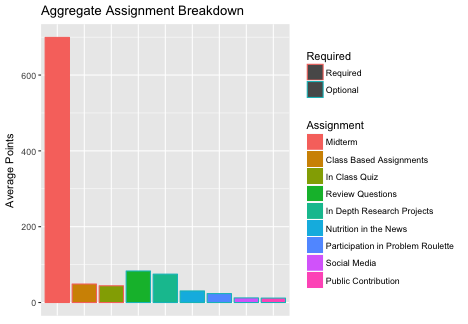
\includegraphics{figures/points-from-assessments-summary-1.png}

\begin{Shaded}
\begin{Highlighting}[]
\NormalTok{p <-}\StringTok{ }\KeywordTok{ggplot}\NormalTok{(}\KeywordTok{filter}\NormalTok{(assignment.summary.data, Assignment }\OperatorTok{!=}\StringTok{ 'Midterm'}\NormalTok{), }\KeywordTok{aes}\NormalTok{(}\DataTypeTok{y=}\NormalTok{Mean.Points, }\DataTypeTok{x=}\NormalTok{Assignment))}
\NormalTok{p }\OperatorTok{+}\StringTok{ }\KeywordTok{geom_bar}\NormalTok{(}\DataTypeTok{stat=}\StringTok{'identity'}\NormalTok{, }\KeywordTok{aes}\NormalTok{(}\DataTypeTok{fill=}\NormalTok{Assignment,}\DataTypeTok{col=}\NormalTok{Required)) }\OperatorTok{+}\StringTok{ }\KeywordTok{scale_x_discrete}\NormalTok{(}\DataTypeTok{limits =}\NormalTok{ positions) }\OperatorTok{+}\StringTok{   }
\StringTok{  }\KeywordTok{labs}\NormalTok{(}\DataTypeTok{title=}\StringTok{"Aggregate Assignment Breakdown - Excluding Midterm"}\NormalTok{, }\DataTypeTok{y =} \StringTok{"Average Points"}\NormalTok{) }\OperatorTok{+}
\StringTok{  }\KeywordTok{theme}\NormalTok{(}\DataTypeTok{axis.title.x=}\KeywordTok{element_blank}\NormalTok{(),}
        \DataTypeTok{axis.text.x=}\KeywordTok{element_blank}\NormalTok{(),}
        \DataTypeTok{axis.ticks.x=}\KeywordTok{element_blank}\NormalTok{())}
\end{Highlighting}
\end{Shaded}

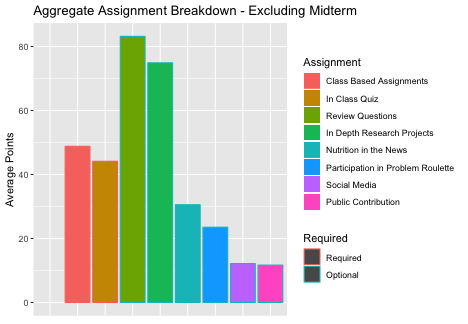
\includegraphics{figures/points-from-assessments-summary-2.png}

\begin{Shaded}
\begin{Highlighting}[]
\NormalTok{p <-}\StringTok{ }\KeywordTok{ggplot}\NormalTok{(assignment.summary.data.relative, }\KeywordTok{aes}\NormalTok{(}\DataTypeTok{y=}\NormalTok{Relative.Points, }\DataTypeTok{x=}\NormalTok{Assignment))}
\NormalTok{p }\OperatorTok{+}\StringTok{ }\KeywordTok{geom_bar}\NormalTok{(}\DataTypeTok{stat=}\StringTok{'identity'}\NormalTok{, }\KeywordTok{aes}\NormalTok{(}\DataTypeTok{fill=}\NormalTok{Assignment,}\DataTypeTok{col=}\NormalTok{Required)) }\OperatorTok{+}\StringTok{ }\KeywordTok{scale_x_discrete}\NormalTok{(}\DataTypeTok{limits =}\NormalTok{ positions) }\OperatorTok{+}\StringTok{   }
\StringTok{  }\KeywordTok{labs}\NormalTok{(}\DataTypeTok{title=}\StringTok{"Aggregate Assignment Breakdown"}\NormalTok{,  }\DataTypeTok{y =} \StringTok{"Points as a Percent of Total"}\NormalTok{) }\OperatorTok{+}
\StringTok{  }\KeywordTok{theme}\NormalTok{(}\DataTypeTok{axis.title.x=}\KeywordTok{element_blank}\NormalTok{(),}
        \DataTypeTok{axis.text.x=}\KeywordTok{element_blank}\NormalTok{(),}
        \DataTypeTok{axis.ticks.x=}\KeywordTok{element_blank}\NormalTok{())}
\end{Highlighting}
\end{Shaded}

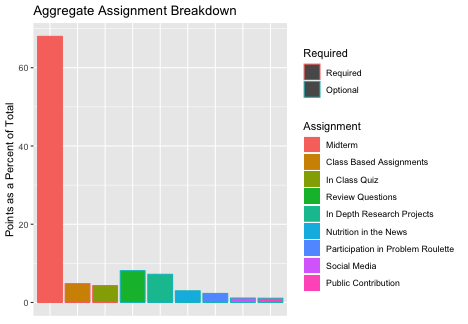
\includegraphics{figures/points-from-assessments-summary-3.png}

\begin{Shaded}
\begin{Highlighting}[]
\NormalTok{p <-}\StringTok{ }\KeywordTok{ggplot}\NormalTok{(}\KeywordTok{filter}\NormalTok{(assignment.summary.data.relative, Assignment }\OperatorTok{!=}\StringTok{ 'Midterm'}\NormalTok{), }\KeywordTok{aes}\NormalTok{(}\DataTypeTok{y=}\NormalTok{Relative.Points, }\DataTypeTok{x=}\NormalTok{Assignment))}
\NormalTok{p }\OperatorTok{+}\StringTok{ }\KeywordTok{geom_bar}\NormalTok{(}\DataTypeTok{stat=}\StringTok{'identity'}\NormalTok{, }\KeywordTok{aes}\NormalTok{(}\DataTypeTok{fill=}\NormalTok{Assignment,}\DataTypeTok{col=}\NormalTok{Required)) }\OperatorTok{+}\StringTok{ }\KeywordTok{scale_x_discrete}\NormalTok{(}\DataTypeTok{limits =}\NormalTok{ positions) }\OperatorTok{+}\StringTok{   }
\StringTok{  }\KeywordTok{labs}\NormalTok{(}\DataTypeTok{title=}\StringTok{"Aggregate Assignment Breakdown - Excluding Midterm"}\NormalTok{, }\DataTypeTok{y =} \StringTok{"Points as a Percent of Total"}\NormalTok{) }\OperatorTok{+}
\StringTok{  }\KeywordTok{theme}\NormalTok{(}\DataTypeTok{axis.title.x=}\KeywordTok{element_blank}\NormalTok{(),}
        \DataTypeTok{axis.text.x=}\KeywordTok{element_blank}\NormalTok{(),}
        \DataTypeTok{axis.ticks.x=}\KeywordTok{element_blank}\NormalTok{())}
\end{Highlighting}
\end{Shaded}

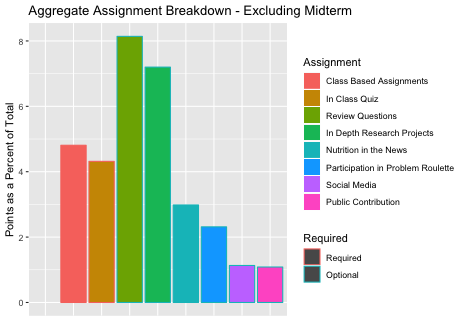
\includegraphics{figures/points-from-assessments-summary-4.png}

\begin{Shaded}
\begin{Highlighting}[]
\KeywordTok{kable}\NormalTok{(assignment.summary.data.required, }\DataTypeTok{caption=}\StringTok{"Average total points"}\NormalTok{)}
\end{Highlighting}
\end{Shaded}

\begin{longtable}[]{@{}lrrrr@{}}
\caption{Average total points}\tabularnewline
\toprule
Required & Median.Points & Median.Points.SD & Relative.Points &
Relative.Points.SD\tabularnewline
\midrule
\endfirsthead
\toprule
Required & Median.Points & Median.Points.SD & Relative.Points &
Relative.Points.SD\tabularnewline
\midrule
\endhead
Required & 799 & 94.7 & 77.8 & 9.22\tabularnewline
Optional & 228 & 69.1 & 22.2 & 6.73\tabularnewline
\bottomrule
\end{longtable}

\begin{Shaded}
\begin{Highlighting}[]
\KeywordTok{kable}\NormalTok{(assignment.summary.data, }\DataTypeTok{caption=}\StringTok{"Average total points per assignment"}\NormalTok{)}
\end{Highlighting}
\end{Shaded}

\begin{longtable}[]{@{}lrrl@{}}
\caption{Average total points per assignment}\tabularnewline
\toprule
Assignment & Mean.Points & SD.Points & Required\tabularnewline
\midrule
\endfirsthead
\toprule
Assignment & Mean.Points & SD.Points & Required\tabularnewline
\midrule
\endhead
Midterm & 699.3 & 91.72 & Required\tabularnewline
Class Based Assignments & 48.8 & 2.10 & Required\tabularnewline
In Class Quiz & 44.1 & 4.56 & Required\tabularnewline
Review Questions & 83.2 & 22.84 & Optional\tabularnewline
In Depth Research Projects & 74.9 & 47.25 & Optional\tabularnewline
Nutrition in the News & 30.5 & 20.60 & Optional\tabularnewline
Participation in Problem Roulette & 23.5 & 9.34 &
Optional\tabularnewline
Social Media & 12.2 & 17.78 & Optional\tabularnewline
Public Contribution & 11.7 & 23.19 & Optional\tabularnewline
\bottomrule
\end{longtable}

\begin{Shaded}
\begin{Highlighting}[]
\KeywordTok{kable}\NormalTok{(assignment.summary.data.relative, }\DataTypeTok{caption=}\StringTok{"Average Relative points per assignment as a percent of total"}\NormalTok{)}
\end{Highlighting}
\end{Shaded}

\begin{longtable}[]{@{}lrrl@{}}
\caption{Average Relative points per assignment as a percent of
total}\tabularnewline
\toprule
Assignment & Relative.Points & SD.Relative.Points &
Required\tabularnewline
\midrule
\endfirsthead
\toprule
Assignment & Relative.Points & SD.Relative.Points &
Required\tabularnewline
\midrule
\endhead
Midterm & 68.02 & 5.766 & Required\tabularnewline
Class Based Assignments & 4.81 & 0.633 & Required\tabularnewline
In Class Quiz & 4.32 & 0.450 & Required\tabularnewline
Review Questions & 8.14 & 2.371 & Optional\tabularnewline
In Depth Research Projects & 7.20 & 4.604 & Optional\tabularnewline
Nutrition in the News & 2.98 & 2.020 & Optional\tabularnewline
Participation in Problem Roulette & 2.31 & 0.921 &
Optional\tabularnewline
Social Media & 1.13 & 1.629 & Optional\tabularnewline
Public Contribution & 1.08 & 2.142 & Optional\tabularnewline
\bottomrule
\end{longtable}

\subsubsection{Student Level}\label{student-level}

\begin{Shaded}
\begin{Highlighting}[]
\NormalTok{assessment.dataset}\OperatorTok{$}\NormalTok{Username <-}\StringTok{ }\KeywordTok{fct_relevel}\NormalTok{(assessment.dataset}\OperatorTok{$}\NormalTok{Username, summary.dataset}\OperatorTok{$}\NormalTok{Username)  }
\NormalTok{assessment.dataset}\OperatorTok{$}\NormalTok{Assignment <-}\StringTok{ }\KeywordTok{fct_relevel}\NormalTok{(assessment.dataset}\OperatorTok{$}\NormalTok{Assignment, positions)}

\NormalTok{p <-}\StringTok{ }\KeywordTok{ggplot}\NormalTok{(assessment.dataset, }\KeywordTok{aes}\NormalTok{(}\DataTypeTok{y=}\NormalTok{Points,}\DataTypeTok{x=}\NormalTok{Username))}

\NormalTok{p }\OperatorTok{+}\StringTok{ }\KeywordTok{geom_bar}\NormalTok{(}\DataTypeTok{stat=}\StringTok{'identity'}\NormalTok{, }\KeywordTok{aes}\NormalTok{(}\DataTypeTok{fill=}\NormalTok{Assignment)) }\OperatorTok{+}
\StringTok{  }\KeywordTok{labs}\NormalTok{(}\DataTypeTok{title=}\StringTok{"Student Level Assignment Breakdown"}\NormalTok{) }\OperatorTok{+}
\StringTok{  }\KeywordTok{theme}\NormalTok{(}\DataTypeTok{axis.title.x=}\KeywordTok{element_blank}\NormalTok{(),}
        \DataTypeTok{axis.text.x=}\KeywordTok{element_blank}\NormalTok{(),}
        \DataTypeTok{axis.ticks.x=}\KeywordTok{element_blank}\NormalTok{()) }\OperatorTok{+}
\StringTok{    }\KeywordTok{geom_hline}\NormalTok{(}\KeywordTok{aes}\NormalTok{(}\DataTypeTok{yintercept=}\DecValTok{1000}\NormalTok{), }\DataTypeTok{color=}\StringTok{"black"}\NormalTok{, }\DataTypeTok{linetype=}\StringTok{"dashed"}\NormalTok{, }\DataTypeTok{size=}\FloatTok{0.5}\NormalTok{) }
\end{Highlighting}
\end{Shaded}

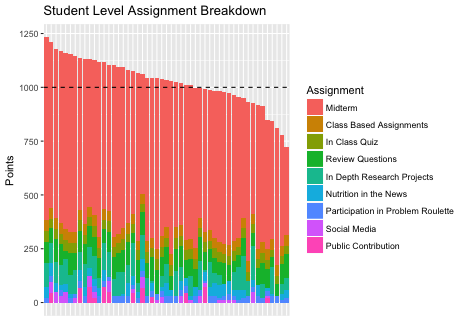
\includegraphics{figures/points-from-assessments-individual-1.png}

\begin{Shaded}
\begin{Highlighting}[]
\NormalTok{assessment.dataset.required <-}
\StringTok{  }\NormalTok{assessment.dataset }\OperatorTok\StringTok{ }
\StringTok{  }\KeywordTok{mutate}\NormalTok{(}\DataTypeTok{Required =} \KeywordTok{ifelse}\NormalTok{(Assignment }\OperatorTok\StringTok{ }\NormalTok{required.assignments, }\StringTok{"Required"}\NormalTok{, }\StringTok{"Optional"}\NormalTok{)) }\OperatorTok
\StringTok{  }\KeywordTok{group_by}\NormalTok{(Username, Required) }\OperatorTok
\StringTok{  }\KeywordTok{summarise}\NormalTok{(}\DataTypeTok{Points =} \KeywordTok{sum}\NormalTok{(Points)) }\OperatorTok
\StringTok{  }\KeywordTok{spread}\NormalTok{(Required, Points) }\OperatorTok
\StringTok{  }\KeywordTok{mutate}\NormalTok{(}\DataTypeTok{Total.Points =}\NormalTok{ Required }\OperatorTok{+}\StringTok{ }\NormalTok{Optional)}
  
\NormalTok{lm.points <-}\StringTok{ }\KeywordTok{lm}\NormalTok{(Optional }\OperatorTok{~}\StringTok{ }\NormalTok{Required, }\DataTypeTok{data=}\NormalTok{assessment.dataset.required)  }
\KeywordTok{par}\NormalTok{(}\DataTypeTok{mfrow=}\KeywordTok{c}\NormalTok{(}\DecValTok{2}\NormalTok{,}\DecValTok{2}\NormalTok{))}
\KeywordTok{plot}\NormalTok{(lm.points)}
\end{Highlighting}
\end{Shaded}

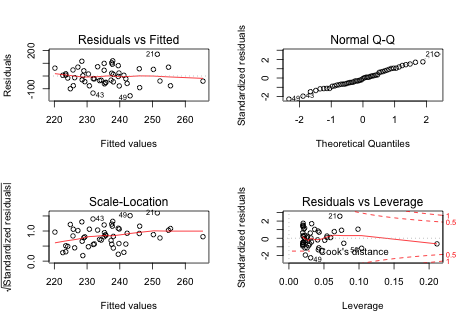
\includegraphics{figures/required-optional-correlations-1.png}

\begin{Shaded}
\begin{Highlighting}[]
\KeywordTok{library}\NormalTok{(broom)}
\KeywordTok{kable}\NormalTok{(}\KeywordTok{tidy}\NormalTok{(lm.points), }\DataTypeTok{caption=}\StringTok{"Linear model of optional points dependent on required points per student."}\NormalTok{)}
\end{Highlighting}
\end{Shaded}

\begin{longtable}[]{@{}lrrrr@{}}
\caption{Linear model of optional points dependent on required points
per student.}\tabularnewline
\toprule
term & estimate & std.error & statistic & p.value\tabularnewline
\midrule
\endfirsthead
\toprule
term & estimate & std.error & statistic & p.value\tabularnewline
\midrule
\endhead
(Intercept) & 315.4 & 82.356 & 3.830 & 0.000\tabularnewline
Required & -0.1 & 0.103 & -0.971 & 0.336\tabularnewline
\bottomrule
\end{longtable}

\begin{Shaded}
\begin{Highlighting}[]
\NormalTok{shapiro.tidy <-}\StringTok{ }\ControlFlowTok{function}\NormalTok{(x) }\KeywordTok{tidy}\NormalTok{(}\KeywordTok{shapiro.test}\NormalTok{(x))}

\KeywordTok{kable}\NormalTok{(}\KeywordTok{with}\NormalTok{(assessment.dataset.required, }\KeywordTok{rbind}\NormalTok{(}\DataTypeTok{Optional =} \KeywordTok{shapiro.tidy}\NormalTok{(Optional), }
                                              \DataTypeTok{Required=}\KeywordTok{shapiro.tidy}\NormalTok{(Required),}
                                              \DataTypeTok{Total.Points =} \KeywordTok{shapiro.tidy}\NormalTok{(Total.Points))), }\DataTypeTok{caption=}\StringTok{"Shapiro-Wilk tests for normality"}\NormalTok{)}
\end{Highlighting}
\end{Shaded}

\begin{longtable}[]{@{}lrrl@{}}
\caption{Shapiro-Wilk tests for normality}\tabularnewline
\toprule
& statistic & p.value & method\tabularnewline
\midrule
\endfirsthead
\toprule
& statistic & p.value & method\tabularnewline
\midrule
\endhead
Optional & 0.986 & 0.785 & Shapiro-Wilk normality test\tabularnewline
Required & 0.953 & 0.042 & Shapiro-Wilk normality test\tabularnewline
Total.Points & 0.970 & 0.225 & Shapiro-Wilk normality
test\tabularnewline
\bottomrule
\end{longtable}

\begin{Shaded}
\begin{Highlighting}[]
\CommentTok{#correlations}
\KeywordTok{kable}\NormalTok{(}\KeywordTok{tidy}\NormalTok{(}\KeywordTok{with}\NormalTok{(assessment.dataset.required, }\KeywordTok{cor.test}\NormalTok{(Optional, Required,}\DataTypeTok{method=}\StringTok{"spearman"}\NormalTok{)), }\DataTypeTok{caption=}\StringTok{"Correlation between optional and required points.  Spearman is used due to lack of normality of the required points distribution."}\NormalTok{))}
\end{Highlighting}
\end{Shaded}

\begin{longtable}[]{@{}rrrll@{}}
\toprule
estimate & statistic & p.value & method & alternative\tabularnewline
\midrule
\endhead
-0.07 & 23657 & 0.623 & Spearman's rank correlation rho &
two.sided\tabularnewline
\bottomrule
\end{longtable}

\begin{Shaded}
\begin{Highlighting}[]
\KeywordTok{kable}\NormalTok{(}\KeywordTok{tidy}\NormalTok{(}\KeywordTok{with}\NormalTok{(assessment.dataset.required, }\KeywordTok{cor.test}\NormalTok{(Optional, Total.Points,}\DataTypeTok{method=}\StringTok{"pearson"}\NormalTok{)), }\DataTypeTok{caption=}\StringTok{"Correlation between optional and total points."}\NormalTok{))}
\end{Highlighting}
\end{Shaded}

\begin{longtable}[]{@{}rrrrrrll@{}}
\toprule
estimate & statistic & p.value & parameter & conf.low & conf.high &
method & alternative\tabularnewline
\midrule
\endhead
0.513 & 4.18 & 0 & 49 & 0.277 & 0.691 & Pearson's product-moment
correlation & two.sided\tabularnewline
\bottomrule
\end{longtable}

\begin{Shaded}
\begin{Highlighting}[]
\NormalTok{p <-}\StringTok{ }\KeywordTok{ggplot}\NormalTok{(assessment.dataset.required, }\KeywordTok{aes}\NormalTok{(}\DataTypeTok{y=}\NormalTok{Optional,}\DataTypeTok{x=}\NormalTok{Required))}
\NormalTok{p }\OperatorTok{+}\StringTok{ }\KeywordTok{geom_point}\NormalTok{() }\OperatorTok{+}
\StringTok{  }\KeywordTok{geom_smooth}\NormalTok{(}\DataTypeTok{method=}\StringTok{'lm'}\NormalTok{) }\OperatorTok{+}
\StringTok{  }\KeywordTok{labs}\NormalTok{(}\DataTypeTok{y=}\StringTok{"Optional Points"}\NormalTok{, }\DataTypeTok{x=}\StringTok{"Required Points"}\NormalTok{) }\OperatorTok{+}
\StringTok{  }\KeywordTok{geom_rug}\NormalTok{(}\DataTypeTok{alpha=}\FloatTok{0.5}\NormalTok{)}
\end{Highlighting}
\end{Shaded}

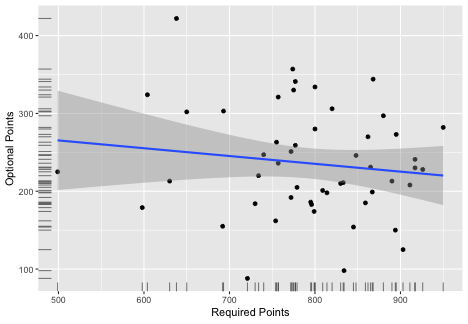
\includegraphics{figures/required-optional-correlations-2.png}

\begin{Shaded}
\begin{Highlighting}[]
\NormalTok{p <-}\StringTok{ }\KeywordTok{ggplot}\NormalTok{(assessment.dataset.required, }\KeywordTok{aes}\NormalTok{(}\DataTypeTok{y=}\NormalTok{Total.Points,}\DataTypeTok{x=}\NormalTok{Optional))}
\NormalTok{p }\OperatorTok{+}\StringTok{ }\KeywordTok{geom_point}\NormalTok{() }\OperatorTok{+}
\StringTok{  }\KeywordTok{geom_smooth}\NormalTok{(}\DataTypeTok{method=}\StringTok{'lm'}\NormalTok{) }\OperatorTok{+}
\StringTok{  }\KeywordTok{labs}\NormalTok{(}\DataTypeTok{y=}\StringTok{"Total Points"}\NormalTok{, }\DataTypeTok{x=}\StringTok{"Optional Points"}\NormalTok{) }\OperatorTok{+}
\StringTok{  }\KeywordTok{geom_hline}\NormalTok{(}\DataTypeTok{yintercept =} \DecValTok{1000}\NormalTok{, }\DataTypeTok{lty=}\DecValTok{2}\NormalTok{,}\DataTypeTok{col=}\StringTok{"red"}\NormalTok{) }\OperatorTok{+}
\StringTok{  }\KeywordTok{geom_rug}\NormalTok{(}\DataTypeTok{alpha=}\FloatTok{0.5}\NormalTok{)}
\end{Highlighting}
\end{Shaded}

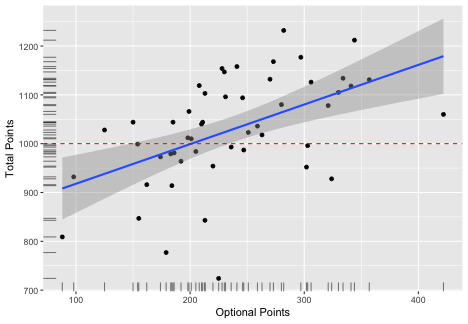
\includegraphics{figures/required-optional-correlations-3.png}

\section{Session Information}\label{session-information}

\begin{Shaded}
\begin{Highlighting}[]
\KeywordTok{sessionInfo}\NormalTok{()}
\end{Highlighting}
\end{Shaded}

\begin{verbatim}
## R version 3.4.2 (2017-09-28)
## Platform: x86_64-apple-darwin15.6.0 (64-bit)
## Running under: macOS High Sierra 10.13.3
## 
## Matrix products: default
## BLAS: /Library/Frameworks/R.framework/Versions/3.4/Resources/lib/libRblas.0.dylib
## LAPACK: /Library/Frameworks/R.framework/Versions/3.4/Resources/lib/libRlapack.dylib
## 
## locale:
## [1] en_US.UTF-8/en_US.UTF-8/en_US.UTF-8/C/en_US.UTF-8/en_US.UTF-8
## 
## attached base packages:
## [1] stats     graphics  grDevices utils     datasets  methods   base     
## 
## other attached packages:
## [1] broom_0.4.3   forcats_0.2.0 ggplot2_2.2.1 bindrcpp_0.2  tidyr_0.7.2  
## [6] dplyr_0.7.4   readr_1.1.1   knitr_1.17   
## 
## loaded via a namespace (and not attached):
##  [1] Rcpp_0.12.14     compiler_3.4.2   plyr_1.8.4       highr_0.6       
##  [5] bindr_0.1        tools_3.4.2      digest_0.6.12    evaluate_0.10.1 
##  [9] tibble_1.3.4     gtable_0.2.0     nlme_3.1-131     lattice_0.20-35 
## [13] pkgconfig_2.0.1  rlang_0.1.4      psych_1.7.8      parallel_3.4.2  
## [17] yaml_2.1.15      stringr_1.2.0    hms_0.4.0        rprojroot_1.2   
## [21] grid_3.4.2       tidyselect_0.2.3 glue_1.2.0       R6_2.2.2        
## [25] foreign_0.8-69   rmarkdown_1.8    reshape2_1.4.2   purrr_0.2.4     
## [29] magrittr_1.5     backports_1.1.1  scales_0.5.0     htmltools_0.3.6 
## [33] mnormt_1.5-5     assertthat_0.2.0 colorspace_1.3-2 labeling_0.3    
## [37] stringi_1.1.6    lazyeval_0.2.1   munsell_0.4.3
\end{verbatim}


\end{document}
